\documentclass[12pt,a4paper]{article}

% Packages
\usepackage{geometry}
\geometry{margin=1in}
\usepackage{fancyhdr}
\usepackage{titlesec}
\usepackage{listings}
\usepackage{xcolor}
\usepackage{graphicx}

% Header & Footer
\pagestyle{fancy}
\fancyhf{}
\rhead{DBT - Assignment 4}
\lhead{Kamithkar Vinod}
\cfoot{\thepage}

% Title formatting
\titleformat{\section}{\large\bfseries}{Problem \thesection:}{0.5em}{}
\titleformat{\subsection}[runin]{\bfseries}{Code:}{0.5em}{}[---]
\titleformat{\subsubsection}[runin]{\bfseries}{Output:}{0.5em}{}[---]

% SQL language definition for listings
\lstdefinelanguage{SQL}{
  morekeywords={
    SELECT, FROM, WHERE, GROUP, BY, ORDER, ASC, DESC, JOIN, ON, AS,
    AND, OR, NOT, IN, IS, NULL, LIKE, HAVING, COUNT, SUM, AVG, MIN, MAX,
    CREATE, TABLE, INSERT, INTO, VALUES, UPDATE, SET, DELETE, DISTINCT,
    CASE, WHEN, THEN, ELSE, END, BETWEEN, EXISTS, UNION, ALL, ANY, LEFT,
    RIGHT, INNER, OUTER, LIMIT, OFFSET, PROCEDURE, BEGIN, FUNCTION, END, RETURNS, RETURN
  },
  sensitive=false,
  morecomment=[l]{--},
  morestring=[b]',
}

\lstset{
    language=SQL,
    basicstyle=\ttfamily\small,
    keywordstyle=\color{blue}\bfseries,
    commentstyle=\color{gray}\itshape,
    stringstyle=\color{red},
    showstringspaces=false,
    frame=single,
    breaklines=true,
    numbers=none
}

% Document Start
\begin{document}

% Title Page
\begin{center}
    \LARGE \textbf{Assignment - 4} \\[0.5cm]
    \Large \textbf{DBMS} \\[1cm]

    \begin{tabular}{rl}
        \textbf{Name:} & Kamithkar Vinod \\
        \textbf{Course:} & PG DAC AUGUST 2025 \\
        \textbf{PRN:} & 250850320040 \\
        \textbf{Form No:} & 250500480 \\
        \textbf{Date:} & 23-10-2025 \\
    \end{tabular}
\end{center}

\vspace{1cm}
\hrule
\vspace{0.5cm}

% Problems

% 1
\section{}
\textbf{Task:} Write a function to return the total number of books in stock.

\subsection{}
\begin{lstlisting}
delimiter //
create function totalBooksInStock()
returns int deterministic
begin
	declare total int default 0;
    select sum(stock) into total
    from books;
    return total;
end //
delimiter ;

select totalBooksInStock() as TotalStock;
\end{lstlisting}

\subsubsection{}
\begin{center}
    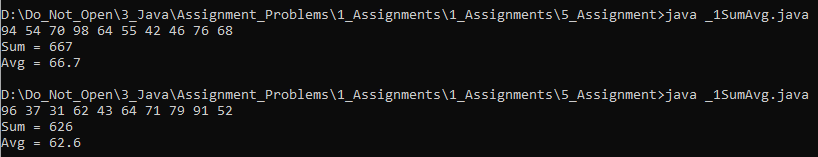
\includegraphics[width=0.8\textwidth]{1.png}
\end{center}

% 2

\section{}
\textbf{Task:} Write a function to return the price of a given book title.

\subsection{}
\begin{lstlisting}

delimiter //
create function priceOfBookTitle(t varchar(50))
returns decimal(10,2) deterministic
begin
	declare priceBook decimal(10, 2) default 0;
    select price into priceBook
    from books where title = t;
    
    return priceBook;
end //
delimiter ;

select priceOfBookTitle('2 States');
\end{lstlisting}

\subsubsection{}
\begin{center}
    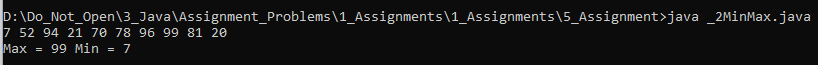
\includegraphics[width=0.8\textwidth]{2.png}
\end{center}

% 3

\section{}
\textbf{Task:} Write a function to find how many books an author has written.

\subsection{}
\begin{lstlisting}
drop function BookByAuthor;

delimiter //
create function BookByAuthor(authorName varchar(50))
returns int deterministic
begin
	declare bookCount int default 0;
    
    select count(b.book_id) into bookCount
    from books b
    join authors a on b.author_id = a.author_id
    where a.author_name = authorName;
    
    return bookCount;
end //
delimiter ;


select BookByAuthor('Chetan Bhagat') as Total_Books;
\end{lstlisting}

\subsubsection{}
\begin{center}
    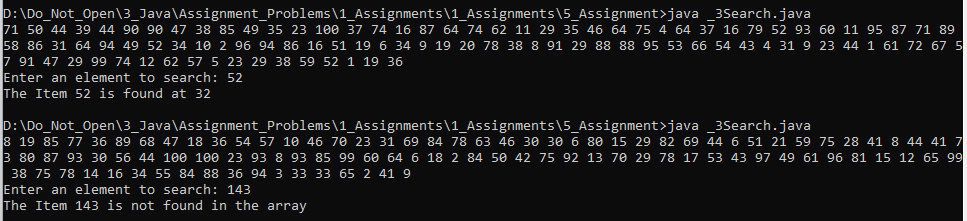
\includegraphics[width=0.8\textwidth]{3.png}
\end{center}

% 4

\section{}
\textbf{Task:} Write a function to return whether a book is "Old" or "New" based on its published year(before 2000 → Old, else → New).

\subsection{}
\begin{lstlisting}
delimiter //
create function CheckBookOldNew(bookTitle varchar(50))
returns varchar(10) deterministic
begin
	declare yearPublished int;
    declare status varchar(50);
    
    select published_year into yearPublished
    from books where title = bookTitle;
    
    if yearPublished < 2000 then
		set status = 'OLD';
	else
		set status = 'NEW';
	end if;
    
    return status;
end //
delimiter ;

select CheckBookOldNew('Harry Potter') AS Book_Status;

select CheckBookOldNew('Five Point Someone') AS Book_Status;

select * from books;
\end{lstlisting}

\subsubsection{}
\begin{center}
    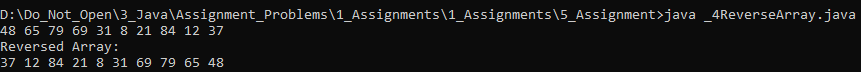
\includegraphics[width=0.8\textwidth]{4.png}
\end{center}

% 5

\section{}
\textbf{Task:} Write a function to calculate a 10% discount on the price of a given book.

\subsection{}
\begin{lstlisting}
delimiter //
create function discountPrice(bookTitle varchar(50))
returns decimal(10, 2) deterministic
begin
	declare bookPrice decimal(10, 2);
    
    select price into bookPrice
    from books where title = bookTitle;
    
    return bookPrice - (bookPrice * 10/100);
end //
delimiter ;

select discountPrice('2 States') as FinalPriceBook;
\end{lstlisting}

\subsubsection{}
\begin{center}
    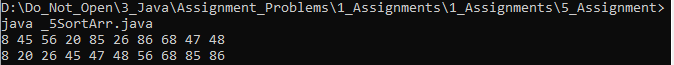
\includegraphics[width=0.8\textwidth]{5.png}
\end{center}

% 6

\section{}
\textbf{Task:} Write a function to return the author's country for a given book.

\subsection{}
\begin{lstlisting}

delimiter //
create function authorCountry(bookName varchar(50))
returns varchar(50) deterministic
begin
	declare a_c_name varchar(50);
    
    select a.country into a_c_name
    from books b 
    join authors a on b.author_id = a.author_id
    where title = bookName;
    
    return a_c_name;
end //
delimiter ;

select authorCountry('Malgudi Days') as AuthorCountry;
select * from authors;
select * from books;
\end{lstlisting}

\subsubsection{}
\begin{center}
    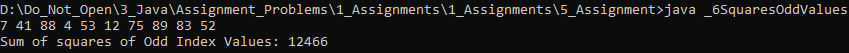
\includegraphics[width=0.8\textwidth]{6.png}
\end{center}

% 7

\section{}
\textbf{Task:} Write a function to find the total value of all books in stock (price × stock).

\subsection{}
\begin{lstlisting}
delimiter //
create function totalValue()
returns decimal(10, 2) deterministic

begin
	declare t_price decimal(10, 2);
    declare t_stock int;
    
    select sum(price) into t_price
        from books;
        
	select sum(stock) into t_stock
        from books;
        
	return t_price * t_stock;
        
end //
delimiter ;

select totalValue() as TotalValueOfAllBooks;
\end{lstlisting}

\subsubsection{}
\begin{center}
    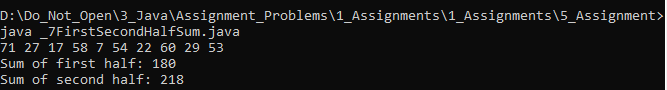
\includegraphics[width=0.8\textwidth]{7.png}
\end{center}

% 8

\section{}
\textbf{Task:} Write a function to return the oldest book title in the store.

\subsection{}
\begin{lstlisting}
drop function OldestBook;
delimiter //
create function OldestBook()
returns varchar(50) deterministic
begin
	declare oldBook varchar(50);
    
    select title into oldBook 
    from books where published_year = (select min(published_year) from books);
    
    return oldBook;
end //
delimiter ;

select OldestBook() as OldestBookInBookStore;
\end{lstlisting}

\subsubsection{}
\begin{center}
    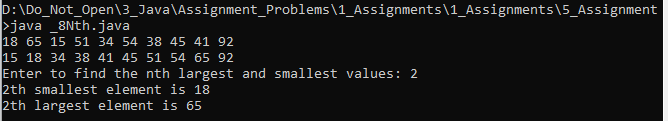
\includegraphics[width=0.8\textwidth]{8.png}
\end{center}

% 9

\section{}
\textbf{Task:} Write a function to check if a given book is in stock or not.

\subsection{}
\begin{lstlisting}
delimiter //
create function IsBookInStock(bookTitle varchar(50))
returns varchar(50) deterministic
begin
	declare availble_stock int;
	declare status varchar(50);
    
    select stock into availble_stock 
    from books where title = bookTitle;
    
    if availble_stock > 0 then
		set status = 'In Stock';
	else
		set status = 'Out of Stock';
	end if;
    
    return status;
end //
delimiter ;

select IsBookInStock('Harry Potter');
\end{lstlisting}

\subsubsection{}
\begin{center}
    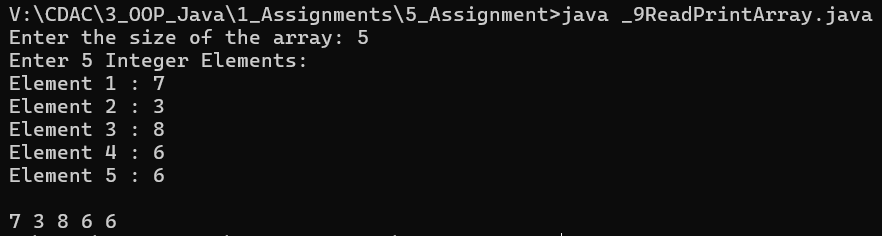
\includegraphics[width=0.8\textwidth]{9.png}
\end{center}

% 10

\section{}
\textbf{Task:} Write a function to return the total number of books available by authors from a specific country.

\subsection{}
\begin{lstlisting}
DELIMITER $$

CREATE FUNCTION TotalBooksByCountry(authorCountry VARCHAR(30))
RETURNS INT
DETERMINISTIC
BEGIN
    DECLARE total_books INT;

    SELECT SUM(b.stock) 
    INTO total_books
    FROM books b
    JOIN authors a ON b.author_id = a.author_id
    WHERE a.country = authorCountry;

    -- If no authors found from that country, return 0 instead of NULL
    IF total_books IS NULL THEN
        SET total_books = 0;
    END IF;

    RETURN total_books;
END $$

DELIMITER ;

SELECT TotalBooksByCountry('India') AS Total_Books_In_Stock;
\end{lstlisting}

\subsubsection{}
\begin{center}
    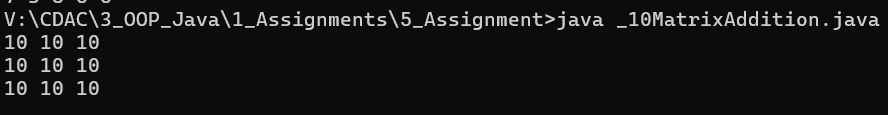
\includegraphics[width=0.8\textwidth]{10.png}
\end{center}


\end{document}
